%%
%% 2019 07 04 Ph. G. Freimann
%%

\section{Ähnlichkeit}\index{Ähnlichkeit}
\sectuntertitel{Treffen sich zwei Parallele.}
%%%%%%%%%%%%%%%%%%%%%%%%%%%%%%%%%%%%%%%%%%%%%%%%%%%%%%%%%%%%%%%%%%%%%%%%%%%%%%%%%

\subsection*{Lernziele}

\begin{itemize}
\item Streckungsfaktor (Ähnlichkeitsfaktor)
\item Translation
\item Drehung
\item Streckung
\item Spiegelung
%%\item Scherung (Lernziel ???)
\end{itemize}
\TadBMTG{72}{5.3}

\newpage


\subsection{Definition Ähnlichkeit}

\bbwCenterGraphic{10cm}{tals/plani/img/aehnlichkeit.png}

%%\raisebox{-2cm}{\includegraphics[width=11cm]{tals/plani/img/aehnlichkeit.png}}

\begin{definition}{Ähnliche Figuren}{}
  
Proportionalität: Sind zwei Figuren ähnlich, so existiert ein
\textbf{Streckungsfaktor}\index{Streckungsfaktor!Planimetrie}\footnote{Der
  Streckungsfaktor heißt auch Ähnlihkeitsfaktor\index{Ähnlichkeitsfaktor!Planimetrie}.}
$k$, der die Strecken ($a$, $b$, $c$, ...) der Originalfigur
($\mathbb{P}$) auf die Bildfigur ($\mathbb{R}$) «abbildet»:
$$a' = k\cdot{}a; b' = k\cdot{}b; c' = k\cdot{} c; ...$$
Winkel: Zudem stimmen die Figuren in allen entsprechenden Winkel überein.
\end{definition}

Daraus ergibt sich durch Division:
\begin{gesetz}{Streckungsfaktor\index{Streckungsfaktor!Planimetrie}
    = Ähnlichkeitsfaktor\index{Ähnlichkeitsfaktor!Planimetrie}}{}

  Für den Streckungsfaktor $k$ gilt:
  $$k = \frac{a'}{a} = \frac{b'}{b} = \frac{c'}{c} = ...$$
\end{gesetz}

\newpage


Für die Flächen gilt jedoch

\begin{gesetz}{Flächen ähnlicher Figuren}{}
$$\frac{|\mathbb{A'}|}{|\mathbb{A}|} = k^2$$
\end{gesetz}


\subsection*{Aufgaben}
%%\TALSAadBFWG{64ff (zentrische Streckung)}{257. 264. 271. (berechnen)}

Ähnliche Figuren:
\TALSAadBMTG{83}{22.}

%%\TALSAadBFWG{69ff (ähnliche Figuren)}{279. 283. 286. 290.}
Fläche:
\TALSAadBMTG{83ff}{23., 25., 27., 29., 30., 40.}

Kreise:
\TALSAadBMTG{85}{41. und 42.}

%%\TALSAadBFWG{73ff (ähnliche Dreiecke)}{306. 309. 319.}


%%\TALSAadBFWG{81ff (Ähnlichkeit am Kreis)}{338. 340. 341. 342.}

\GESOAadBMTA{???}{???}

